\section{Methodisches Vorgehen zur Problemlösung}

%%%%%%%%%%%%%%%%%%%%%%%%%%%%%%%%%%%%%%%%%%%%%%%%%%%%%%%%%%%%%%%%%%%%%%%%%%%%%%%%%%%%%%%%%%%%%%
\subsection{Aktueller Stand der Technologie}

\subsubsection{Bluetooth-Technologie}\label{sssec:BLE}
Bluetooth ist eine drahtlose Datenübertragunsgtechnologie, die basierend auf der Funktechnik Verbindungen zwischen Geräten über eine kurze Distanz ermöglicht. Im engen Nahbereich gilt Bluetooth als der Kommunikationsstandard \citep[Vgl.][S. 133]{mobil-sicher}. Mit dem Bluetooth Low Energy (BLE \nomenclature{BLE}{\textbf{B}luetooth \textbf{L}ow \textbf{E}nergy}) Standard, der 2009 verabscheidet wurde der Stromverbrauch für eine Bluetooth-Verbindung in den Endgeräten drastisch reduziert. Dies gelang unter anderem durch kürzere Verbindungsaufbauzeiten und Schlafphasen (Standby) zwischen den Sendezyklen. Eine vergleichende Untersuchung zum Energieverbrauch von Bluetooth und BLE veröffentlichten \cite{ble-energy}. 


\subsubsection{Raspberry Pi}\label{sssec:raspberry}
Für die Zentrale und die DeSearch-Boxen ist zunächst eine Hardware-Entscheidung notwendig. Benötigt werden Mikrocontroller oder Mikrocomputer mit folgenden Eigenschaften:
\begin{itemize}
	\item W-LAN Verbindung von der Box zur Zentrale möglich
	\item Bluetooth-fähige Box zur Markenerkennung
	\item Zentrale muss als Server fungieren und HTTP-Requests senden und verarbeiten können
	\item Datenbank-Installation zur Datenhaltung notwendig
\end{itemize}
Zudem sollen die Kosten pro Gerät so gering wie möglich gehalten werden. \\
Der Rasberry Pi ist ein Mikrocomputer mit einer Grundfläche, die etwas größer ist als eine Kreditkarte. In Abbildung \ref{fig:raspi} ist ein Raspberry Pi in der Draufsicht abgebildet.
\begin{figure}
	\centering
	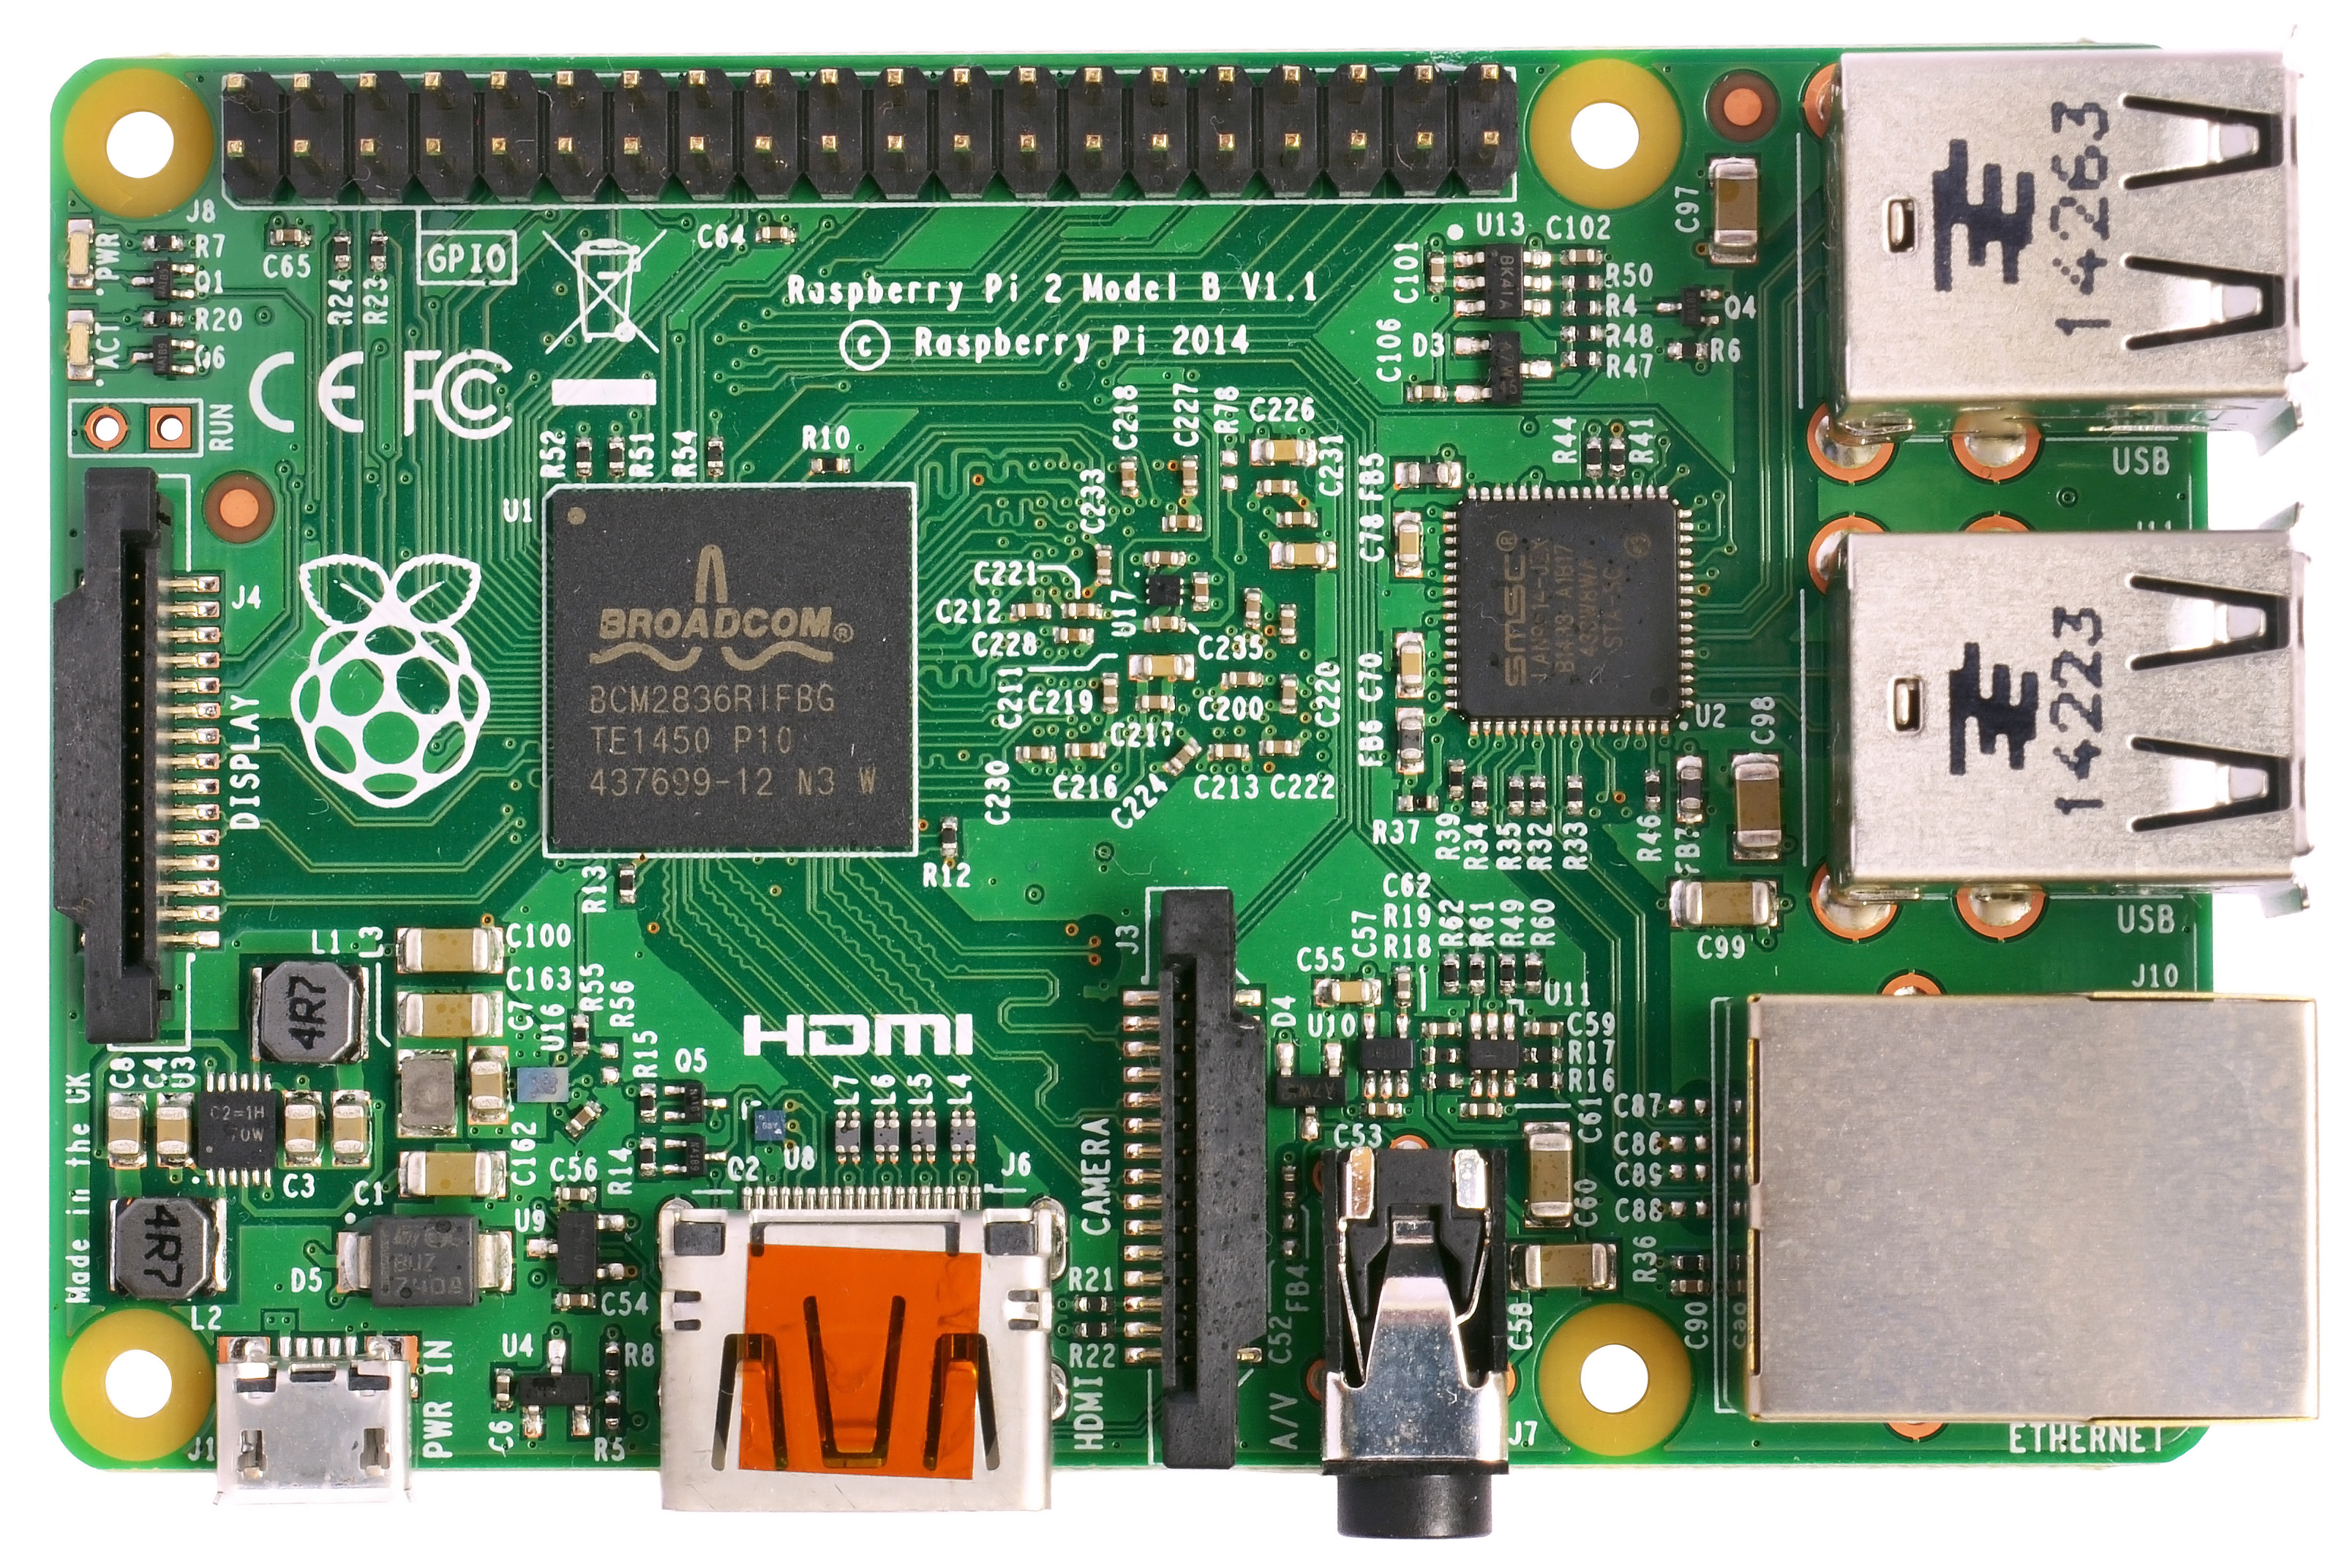
\includegraphics[width=1.0\linewidth]{images/Raspberrypi}
	\caption[Raspberry Pi in der Draufsicht]{Raspberry Pi Model 2, fungiert im DeSearch-Projekt als DeSearch-Box und als Zentrale, Quelle: https://en.wikipedia.org/wiki/Raspberry\_Pi}
	\label{fig:raspi}
\end{figure}
 Die Anschaffungskosten liegen ohne Zubehör bei etwa 42 €. Für diese geringen Anschaffungskosten erhält man einen vollwertigen, Linux-Basierten Computer mit einer ARM-CPU, W-LAN und Bluetooth-Schnittstelle. Im Gegensatz zu Mikrocontrollern ist der Raspberry Pi leistungsfähiger und läuft stabiler \citep[Vgl.][S.35ff.]{raspi}. Auf einem Arduino beispielweise kann nur C++-Code in einer Endlos-Schleife ausgeführt werden. Der Pi hingegen bietet die Möglichkeit, Bash-Skripte, Python-Code, Datenbank-Anfragen und Webserver gleichzeitig auszuführen. Die Entscheidung für den Raspberry Pi ist auch aufgrund der relativ niedrigen Anschaffungskosten für einen kompletten Rechner mit Betriebssystem gefallen. Für die Entwickler ist das Betriebssystem Linux zudem am einfachsten zu bedienen. Für das Projekt werden Pakete mit Raspberry Pi Model 2, SD-Karte, W-LAN und Bluetooth-Dongles, Netzteil und Gehäuse für ca. 75 € pro Paket angeschafft.
\subsubsection{Authentifizierungstechnologie}
\subsubsection{Software-Rollout mit apt und dpgk}
Zum Installieren von Software wird unter Debain basierten System (dazu gehört neben Ubuntu und natürlich Debian selbst auch das Standardbetriebssystem des Raspberry Pi: Rasbian) das Programm "dpkg" verwendet.
Dazu muss eine ".deb" Datei vorliegen. Statt dem manuellen Download, der auch bei jedem Update erneut durchgeführt werden müsste, lässt sich zum Verteilen der deb Dateien apt verwenden.
Apt selbst nimmt keine Installation vor, es kümmert sich lediglich um die Beschaffung der aktuellsten deb Dateien und deren Abhängigkeiten (ebenfalls im deb Format) und reicht diese zur Installation an dpkg weiter.
Neue Programme lassen sich mit "apt-get install <packetname>" installieren.
Dazu hält sich apt eine Liste mit allen verfügbaren Programmen in einem lokalen Cache vor. Um diese Liste zu aktualisieren kann der Befehl "apt-get update" verwendet werden.
Dabei werden alle in der Datei "/etc/sources.list" bzw. dem Ordner "/etc/sources.list.d/" spezifizierten Quellen abgefragt.
Die Quellen werden dabei als URL spezifiziert und können unterschiedlichste Protokolle erfordern.
Beispielsweise HTTP, HTTPS, FTP oder lokale Datenträger.
Zum aktualisieren aller installierten Programme (nach dem ausführen von "apt-get update") wird der Befehl "apt-get upgrade" verwendet. Dabei wird die Softwareliste im Cache mit den installierten Programmen abgeglichen, ist eine aktuellere Version verfügbar wird deren deb Paket heruntergeladen und mittels dpkg installiert.
\newline\textbf{apt}\newline
Zum Aktualisieren der Softwareliste lädt apt zunächst die Release Datei von der Quelle runter, diese ist mit gnupg signiert und enthält Informationen über die Packetquelle wie die unterstützen CPU Architekturen.
Außerdem sind Hash-Summen der Packages Dateien enthalten, da diese nicht gnupg signiert sind.
Danach wir die Package Datei heruntergeladen. Diese Datei ist spezifisch für eine Architektur und kann in einem Repository mehrfach vorkommen.
Sie enthält die Namen aller verfügbaren Pakete dieses Repositories sowie deren Abhängigkeiten, Beschreibung, Pfad und Hash-Werte der zugehörigen deb Datei sowie weitere Metadaten.
\newline\textbf{dpkg}\newline
dpkg installiert, konfiguriert und deinstalliert deb Pakete.
Eine deb Datei enthält in einem Archiv alle Dateien die das zu installierende Programm zur Ausführung benötigt.
Außerdem sind in einem weiteren Archiv verschiedene Kontrolldateien enthalten, eine davon enthält Metadaten wie Namen des Pakets, Abhängigkeiten und der Beschreibung.
Daneben sind (optional) Skripte enthalten die ausgeführt werden bevor oder nachdem das Paket Installiert, Deinstalliert oder Aktualisiert wurde. 

\subsubsection{PostgreSQL}
PostgreSQL ist ein objektrelationales Datenbank-Management-System (DBMS), das aus dem Projekt POSTGRES der kalifornischen Universität Berkeley heraus entstanden ist. Der objektrelationale Ansatz bedeutet eine Erweiterung der relationalen DBMS um die Konzepte der Objektorientierung. Somit können in objektrelationalen DBMS beispielsweise komplexe Datenstrukturen mit Attributen definiert werden oder Vererbungen vorgenommen werden \citep[Vgl.][S. 135f.]{datenbanken}. In anderen DBMS muss hierfür \enquote{object relational mapping} (ORM) hinzugezogen werden, um Objektstrukturen auf relationale Tabellen abzubilden \citep[Vgl.][S. 426]{balzert} Viele Konzepte, die in POSTGRES neu waren, wurden später in kommerzielle DBMS übernommen. PostgreSQL ist die Open-Source-Variante von POSTGRES und unterstützt einen großen Teil des SQL-Standards. Zudem bietet es Features wie komplexe Queries, Fremdschlüsselbeziehungen, Trigger, updatefähige Views und transaktionale Integrität. Außerdem kann der Benutzer PostgreSQL beliebig durch neue Datentypen, Funktionen, Operatoren oder Aggregationsfunktionen erweitern. Aufgrund der Open-Source-Lizenz kann PostgreSQL von jedem verwendet, verbessert oder verteilt werden
\nomenclature{DBMS}{\textbf{D}aten\textbf{b}ank \textbf{M}anagement \textbf{S}ystem}
\citep[Vgl.][preface, S. lxvi]{postgres}. Für das DeSearch-Projekt eignet sich PostgreSQL vor allem wegen seiner Open-Source-Lizenz, was die Kosten für das Projekt gering hält. Zudem ist die Möglichkeit, eigene Datentypen definieren zu können, von Vorteil. Da die Datenbank auf dem Zentral-Raspberry verwendet wird, der meist über SSH in der Konsole bedient wird, ist PostgreSQL einfach zu bedienen, da es über einen Konsolenclienten verfügt.

\subsubsection{Services unter Linux mit systemd}\label{sssec:systemd}
\textbf{systemd} ist ein Init-Tool unter Linux, das als neuere Alternative zu sysvinit und upstart gilt. Es ist für das Starten von Services und Mounten von Hard Disks beim boot zuständig. Systemd verwaltet Hintergrunddienste(Daemons) und bietet ein Event-gesteuertes Starten von diesen, analog zum Runlevel-Prinzip von sysvinit. Dies bedeutet, dass bestimmte Gruppen von Services an bestimmten Punkten beim Boot gestartet werden, zum Beispiel sobald die GUI verfügbar ist oder sobald eine aktive Netzwerkverbindung besteht. In Tabelle \ref{tab:lvl} ist ein Vergleich zwischen den sysvinit-runlevels und den systemd-targets zu sehen. 
\begin{table}[h]
	\begin{tabular}{|p{2,5cm}|p{3,5cm} |p{8,5cm} | }
		\hline
		\textbf{sysvinit Runlevel} & \textbf{systemd-target} & \textbf{Bedeutung}\\ \hline
		0 & poweroff.target & System-Shutdown	\\ \hline
		1, single & rescue.target & Single-User-Modus \\ \hline
		2,4 & multi-user.target & Benutzerdefinierte runlevels, per default identisch mit runlevel 3 \\ \hline
		3 & multi-user.target & Multi-User-Umgebung, ohne graphische Benutzer\-oberfläche (Login über Konsole möglich)\\ \hline
		5 & graphical.target & Multi-User-Umgebung, graphische Benutzer\-oberfläche \\ \hline
		6 & reboot.target & System-Reboot \\ \hline
		emergency & emergency.target & Emergency Shell\\ \hline
		
	\end{tabular}
	\caption[Übersicht über die targets von systemd]{Übersicht über die targets von systemd, in Anlehnung an \cite{fedora}}
	\label{tab:lvl}
\end{table}
Mithilfe dieser targets können beispielsweise voneinander abhängige Hintergrundservices nacheinander gestartet werden. Neben den runlevels entsprechenden targets gibt es noch einige weitere, wie zum Beispiel das \textbf{network-online.target}.
Auch der Raspberry Pi mit Raspbian verwendet systemd. Für die DeSearch-Boxen eignet es sich, um den Scan-Vorgang als Hintergrundprozess zu verwalten und so sicherzugehen, dass dieser stabil läuft und nach eventuellem reboot selbständig wieder startet.\newline
Über die Konsole kann \textbf{systemctl} aufgerufen werden. Dies ist die Überwachungs- und Steuereinheit von systemd. Mit \texttt{systemctl start xyz.service} kann ein Service gestartet werden. Respektive kann mit  \texttt{systemctl restart xyz.service} und \texttt{systemctl stop xyz.service} der Service neugestartet oder angehalten werden. Mit  \texttt{systemctl status xyz.service} wird eine Ausgabe erzeugt, die über den Status des Service informiert und eventuelle Ausgaben des Service anzeigt. Diese Kommandos und alle weiteren Optionen von systemctl befinden sich im Manual \citep[][]{systemctl-man}.

\subsection{Umsetzung der Anforderungen}

\subsubsection{Authentifizierung} \label{cap:authentifizierung}
Im System gibt es 4 verschiedene Authentifizierung (vgl. Tabelle \ref{tab:authentifizierungen}).\newline
Die Zentrale authentifiziert sich bei den Nutzern und Boxen (Authentisierende) mittels SSL Zertifikat, wie jeder Webserver der im Internet über HTTPS zur Verfügung steht. Aktuell handelt es sich dabei um ein selbst signiertes Zertifikat, das auf den Boxen und den Endgeräten der Nutzer manuell eingespielt werden muss. Ist die DeSearch Zentrale zukünftig über eine globale Domain erreichbar, kann auch ein Zertifikat bei einem Root CA beantragt werden, welcher die Browserhersteller vertrauen. \newline
Die Boxen authentifizieren sich gegenüber der Zentrale ebenfalls mittels eines SSL Zertifikates.
Dieses muss beim installieren der Box zwischen Zentrale und Box ausgetauscht werden. Dazu wird auf der Box das Python Script "/opt/desearch-client/keyExchange.py" und der Zentrale die Serverversion des Scripts "/opt/desearch-server/keyExchange.py" mit root Berechtigung gestartet. Daraufhin tauschen Server und Klient ihre Zertifikate aus und zeigen deren Hashwerte an. Die Übereinstimmung ist dann zu prüfen um MITM Attacken auszuschließen. Nach bestätigen der Gleichheit werden die Zertifikate abgespeichert. \newline
Nutzer authentifizieren sich bei der Zentrale mit einer Nutzername / Passwort Kombination. Danach erstellt die Zentrale ein Token, das für alle weiteren Anfragen verwendet wird. Das Token wird selbstverständlich transparent für den Nutzer vom JavaScript Code des Userinterfaces entgegen genommen, verwaltet und mitgesendet.

\begin{table}[h]
	\begin{tabular}{ | l | l | l | l |}
		\hline
		\textbf{Zeile} & \textbf{Authentifizierender} & \textbf{Authentisierender} &  \textbf{Methode} \\ \hline
		1 & Zentrale & Box      & SSL Klient Zertifikat \\ \hline
		2 & Zentrale & Nutzer   & Nutzername, Passwort, Token \\ \hline
		3 & Box      & Zentrale & SSL Server Zertifikat \\ \hline
		4 & Nutzer   & Zentrale & SSL Server Zertifikat \\ \hline
		
	\end{tabular}
	\caption{Authentifizierungen im System}
	\label{tab:authentifizierungen}
\end{table}

\subsubsection{Erkennen der Marken über Bluetooth}
Durch die eingschränkte Sendereichweite von Bluetooth soll die Ortung im DeSearch-Projekt gelingen. Die dementen Patienten tragen kleine BLE-Sendemarken am Körper, die von den fest installierten DeSearch-Boxen erkannt werden, sobald sich der Patient in der Nähe aufhält. So kann auf den ungefähren Aufenthaltsort der Person geschlossen werden, sobald eine der Boxen einen Treffer an die Zentrale meldet. \newline
Als Ergebnis eines studentischen Workshops auf der Hütte in Balderschwang gibt es eine Python Klasse, die einen BLE Scan starten kann und basierend auf einer Liste von MAC Adressen eine Callback-Funktion aufruft, wann immer eine der MAC Adressen in der Liste gesichtet wird.
Diese Klasse verwendet die Bibliothek "bleep", die sich allerdings im Laufe der Projektarbeit als nicht geeignet herausstellte, da sie folgende Probleme aufweist:
\begin{itemize}
	\item Wird sie nicht mit root-Rechten ausgeführt, kommt es zum Absturz.
	\item Die Installation ist für eine großflächige Verteilung zu aufwändig und erfordert unter anderem die Installation einer modifizierten Version von "pygattlib" \citep[Vgl.][]{bleep-installation}.
	\item Es handelt sich dabei um ein Einmannprojekt, dessen Entwickler die Bibliothek aus einem privaten Bedürfnis heraus geschaffen hat. Damit ist die Softwarequalität und Wartung abhängig von einer einzelnen Person.
\end{itemize}
Zur Bluetooth-Kommunikation unter Linux kann der im Linux Kernel enthaltene Bluetooth Stack "bluez" verwendet werden. Dieser enthält auch Treiber für die meisten Bluetooth Chipsets.
Auch die bleep Bibliothek verwendet bluez. Im Rahmen der Projektarbeit erfolgt eine Reimplementierung der Scanner-Klasse in Python, die ohne die Verwendung von bleep auskommt.
In der Reimplementierung wurden dabei die Schnittstellen der Klasse erhalten, die Kommunikation mit bluez findet nun über den DBus statt. Dies erfordert keine root-Rechte und ist neben den Kommandozeilen-Tools der einzig im offiziellen Git-Repository von bluez dokumentierte Weg zum Ansprechen der Schnittstellen \citep[Vgl.][]{bluez-git}. Außerdem werden damit nur noch die DBus-Bibliothek von Python und bluez auf den DeSearch-Boxen benötigt, diese sind in den offiziellen Paketquellen enthalten und damit einfach zu verteilen und zu aktualisieren.

\subsubsection{Robustheit des Systems durch Services}\label{sssec:services}
Um eine gewisse Robustheit des Systems zu gewährleisten, muss sichergestellt werden, dass die Python-Skripte zum Scan auf den DeSearch-Boxen sowie die Python-Skripte des Web-Servers auf der Zentrale immer laufen. Dies wird durch Hintergrundservices realisiert. Anforderung an die Services ist es, dass sie sich nach einem Reboot selbständig starten und nach einem unerwarteten Fehler oder Ausführungs-Stop selbständig re-spawnen(d.h. sich selbst neu-starten). Realisiert wurde dies durch systemd-Services, welche in Kapitel \ref{sssec:systemd} bereits erläutert wurden. Die Konfiguration innerhalb des Service ist für Zentrale und DeSearchBox gleich, da die Anforderungen auch gleich sind. Um einen Hintergrundservice anzulegen, muss zunächst das \texttt{.service}-File unter dem Pfad \texttt{/lib/systemd/system/} angelegt werden. In diesem Verzeichnis werden alle Services von systemd nachgeschlagen. Beispielhaft ist in Abbildung \ref{fig:service} das Service-File der DeSearch-Zentrale zu sehen.
\begin{figure}[bth]
	\centering
	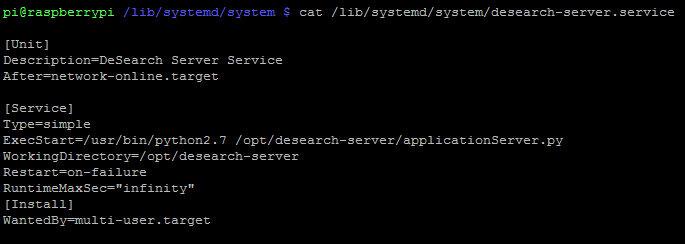
\includegraphics[width=1.0\linewidth]{images/service-systemd}
	\caption[Service-File auf dem Zentral-Pi]{Service-File auf dem Raspberry Pi, der als Zentrale fungiert.}
	\label{fig:service}
\end{figure}
Zunächst werden unter \texttt{[Unit]} Informationen zu dieser Service-Unit aufgeführt. Dies ist die Beschreibung des Service (unter Description) und die Information, wann der Service beim Boot gestartet werden soll. Hier stehen unter Anderem die Optionen \enquote{Before} und \enquote{After} zur Verfügung. Im \texttt{desearch-server.service} wird durch \enquote{After=network-online.target} ausgedrückt, dass der Service erst gestartet werden darf, wenn eine aktive Netzwerkverbindung besteht (siehe auch Kapitel \ref{sssec:systemd}). Ansonsten wird der Start des Service verzögert, bis die angegebene Bedingung erfüllt ist.
In der darauf folgenden \texttt{[Service]}-Sektion wird angegeben, was der Hintergrundservice tun soll. Die Angabe des \enquote{simple}-Type bewirkt, dass der Prozess, den der Service startet, auch dessen Haupt-Prozess ist. Anders verhält es sich, wenn hier \enquote{forking} gewählt wird: Dann verhält sich der Prozess wie ein traditioneller UNIX-Daemon und startet als Kindprozess des Service. \\
Nach der Angabe des Typs wird unter \enquote{ExecStart} angegeben, was der Service ausführen soll. Hier wird zunächst der Pfad der Python-Installation angegeben und anschließend der Pfad des deSearch-Server-Skripts, das von Python ausgeführt werden soll. Zusätzlich wird noch ein Working-Directory angegeben, da Python sonst von dem Service im Root-Verzeichnis gestartet wird und dann die restlichen benötigten Python-Skripte nicht gefunden werden. \\
Der nächste Parameter, \enquote{Restart}, bestimmt wann der Service neu gestartet werden soll. Hier gibt es verschiedene Optionen, die in der man-Page von systemd nachgeschlagen werden können \citep{systemd-service}. Für lang laufende Hintergrundprozesse empfiehlt die man-Page die Wahl von \enquote{Restart=on-failure}. Der Service wird bei unsauberen Exit-Codes (ungleich 0), wenn er von einem Signal beendet wird (z.B. Core Dump), bei einem Timeout oder (falls konfiguriert) bei fehlendem Watchdog-Signal neu gestartet. Die maximale Laufzeit des Service wird zudem im nächsten Argument \enquote{RuntimeMaxSec} auf unendlich gesetzt.\\
Im \texttt{[Install]}-Abschnitt wird abschließend festgelegt, welche Abhängigkeiten ein Service hat. Die Angabe \enquote{multi-user.target} stellt eine Abhängigkeit her, die bewirkt, dass der Service dann gestartet wird, wenn auch die Multi-User-Umgebung gestartet wird. \\
Nach dem Anlegen des Service-Files wird \texttt{systemctl daemon-relaod} einmalig ausgeführt, um anschließend mit \texttt{systemctl enable desearch-server.service} den Service zu aktivieren. Nun kann entweder durch einen reboot der Service automatisch gestartet werden (wie konfiguriert) oder mittels \texttt{systemctl start desearch-server.service} auch manuell. Abbildung \ref{fig:systemctl-status} zeigt die Statusausgabe von Systemctl nach erfolgreichem Start des Service.
\begin{figure}[bth]
	\centering
	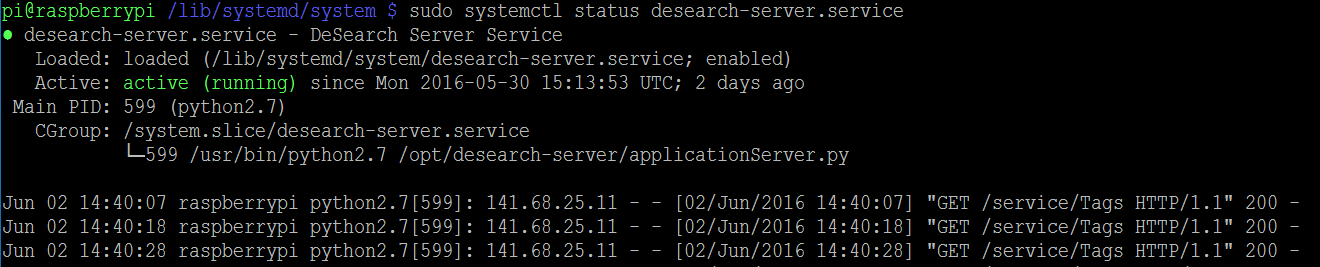
\includegraphics[width=1.0\linewidth]{images/service-status}
	\caption[Status-Ausgabe von Systemctl]{Status-Ausgabe von Systemctl für den deSearch-Zentral-Service.}
	\label{fig:systemctl-status}
\end{figure}

\subsubsection{Datenbankschema}
In Abbildung \ref{img:db-schema} ist das Datenbankschema zu sehen, mit dem die Zentrale arbeitet. 
\begin{figure}
	\centering
	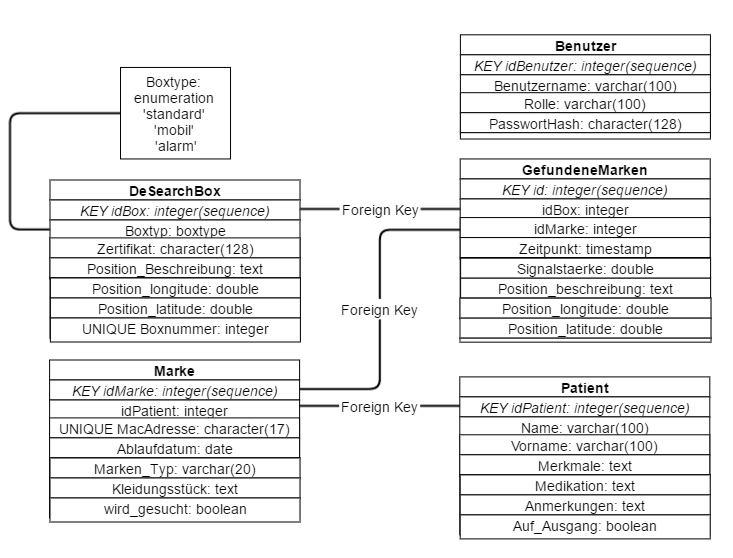
\includegraphics[width=1.0\linewidth]{images/db-schema}
	\caption[Datenbankschema der Zentrale]{Datenbankschema der Zentrale, Quelle: eigene Darstellung}
	\label{img:db-schema}
\end{figure}
\\Für den Zugang zur Web-Oberfläche werden \textbf{Benutzer} mit ihren Rollen in der Datenbank angelegt. Das Passwort wird dabei als Hash mit 128 Zeichen in der Datenbank gespeichert. 
\\Jede \textbf{DeSearch-Box} wird in der Datenbank mit ihrer Position und Boxnummer angelegt. Für die Zukunft wurde bereits das Feld \enquote{Boxtyp} erstellt, da im weiteren Verlauf ortsfeste, mobile und Alarm-Boxen unterschieden werden sollen. Bei mobilen Boxen(z.B. im Auto, in Linienbussen) wird anstatt einer festen Positionsbeschreibung die genaue Geo-Location mit Longitude und Latitude ermittelt. Alarm-Boxen können beispielsweise am Hof-Ausgang oder an der Bushaltestelle installiert werden und standardmäßig immer Alarm auslösen, wenn dort eine Marke gefunden wird.
\\Die \textbf{Marken} werden in der Datenbank mit einer eindeutigen Mac-Adresse abgelegt, die beim Abgleich mit den Scan-Ergebnissen verwendet wird. Außerdem wird die ID des zugehörigen Patienten vermerkt und ein Hinweis auf das jeweilige Kleidungsstück, in das die Marke eingenäht ist. Zusätzlich wird ein Ablaufdatum in die Datenbank eingetragen, das den ungefähren Zeitpunkt des nächsten Batteriewechsels festhält. Somit kann eine Warnmeldung angezeigt werden, wenn der Batteriewechsel fällig ist. Ein wichtiges Feld ist der boolean \enquote{wird\_gesucht}. Wird auf der Web-Oberfläche eine Suche gestartet, so werden alle zu dieser Person gehörigen Marken auf wird\_gesucht gesetzt. Nur dann werden Treffer zu dieser Person von den Boxen an die Zentrale gemeldet. Finden die Suchenden beispielsweise nur ein Kleidungsstück der vermissten Person, können einzelne Marken gezielt von der Suche ausgeschlossen werden. 
\\Ein \textbf{Patient} liegt in der Datenbank mit Name, Vorname und weiteren für die Suche wichtigen Informationen vor. Beispielsweise kann unter Merkmale die Beschreibung einer Person vermerkt werden, unter Medikation und Anmerkungen können wichtige Hinweise im Fall eines Fundes oder einer längeren Abwesenheit der Person gespeichert werden. Gerade bei Diabetikern oder Patienten, die regelmäßig Medikamente nehmen müssen, ist diese Information besonders wichtig. Das Flag \enquote{Auf\_Ausgang} kann gesetzt werden, falls ein Angehöriger mit der Person das Pflegeheim verlässt, beispielsweise für einen Spaziergang. Somit wird ein Fehlalarm verhindert.
\\Die Tabelle \textbf{GefundeneMarken} kann eine Suchaktion protokollieren. Jeder Treffer, den eine Box registriert und an die Zentrale sendet, wird hier dokumentiert. Ein Treffer wird mit der zugehörigen BoxID, der MarkenID, dem Zeitpunkt und der Position in die Datenbank gelegt. Somit können auf der Web-Oberfläche alle Treffer in einer Zeitreihe angezeigt werden. Aus Datenschutzgründen wird diese Tabelle nach jeder abgeschlossenen Suchaktion gelöscht.

\subsubsection{Benutzeroberfläche}\label{sssec:ui}
Die Benutzeroberfläche wurde unter Verwendung des Frameworks Polymer erstellt. Dieses zeichnet sich vor allem dadurch aus, dass es die Erstellung eines "responsive UI", also einer Nutzerschnittstelle, die sich auf Smartphones, Tabletcomputern, Laptops sowie Desktop PC gleichermaßen bedienen lässt, unterstützt.\newline
Nachdem sich der Nutzer eingeloggt hat (vgl. Abbildung \ref{img:ui/login}) sieht er eine Liste aller Patienten im System. Patienten, nach denen aktuell gefahndet wird, werden dabei mit einem roten Icon hervorgehoben (vgl. Abbildung \ref{img:ui/personenliste}). Eine Liste, die nur die gesuchten Patienten enthält, lässt sich über das Menü aufrufen (vgl. Abbildung \ref{img:ui/menu}). \newline
Wählt der Nutzer in einer der Listen einen Patienten aus, so bekommt er weitere Details und verfügbare Aktionen angezeigt. Bei den Details handelt es sich um zuvor hinterlegt Informationen wie das Aussehen und die Anmerkungen sowie die Sichtungen im Falle einer aktiven Fahndung. Verfügbare Aktionen sind das Starten bzw. Stoppen einer Fahndung, das Löschen und Bearbeiten des Patienten und die Verwaltung der Marken starten (vgl. Abbildung \ref{img:ui/persondetails}). \newline
Startet der Nutzer die Markenverwaltung so bekommt er zunächst die für den Patienten hinterlegten Marken aufgelistet und kann diese entfernen oder als gefunden markieren (vgl. Abbildung \ref{img:ui/markenverwalten}). Außerdem hat er die Möglichkeit dem Patienten eine neue Marke zuzuordnen (vgl. Abbildung \ref{img:ui/markehinzufuegen}). \newline
Neue Patienten werden über einen Button in der Liste hinzugefügt. Dieser öffnet ein Dialogfenster (vgl. Abbildung \ref{img:ui/personhinzufuegen}) in dem Details zum Patienten hinterlegt werden können.

\begin{figure}
	\centering
	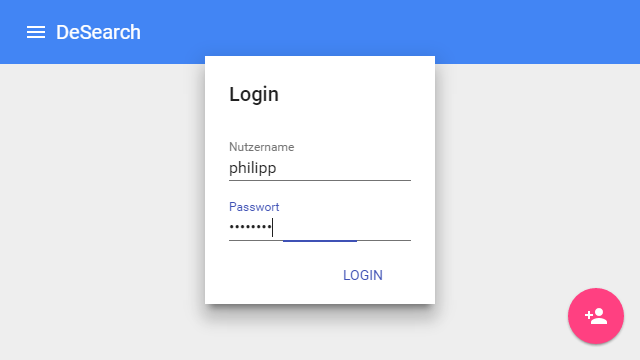
\includegraphics[width=1.0\linewidth]{images/ui/login}
	\caption{Login}
	\label{img:ui/login}
\end{figure}

\begin{figure}
	\centering
	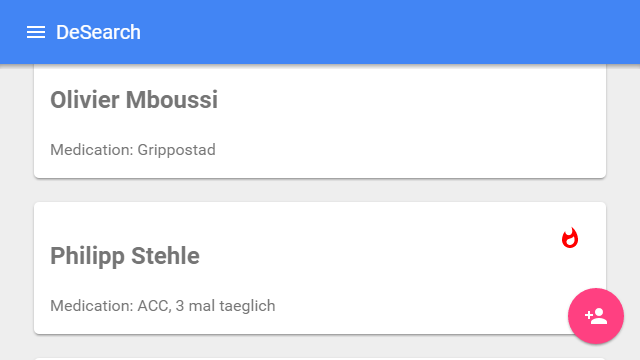
\includegraphics[width=1.0\linewidth]{images/ui/personenliste}
	\caption{Liste aller Patienten}
	\label{img:ui/personenliste}
\end{figure}

\begin{figure}
	\centering
	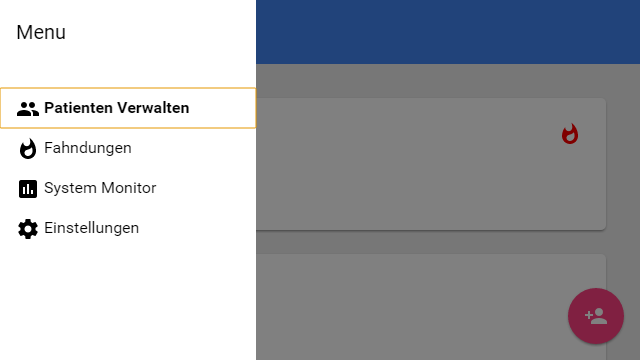
\includegraphics[width=1.0\linewidth]{images/ui/menu}
	\caption{Menü}
	\label{img:ui/menu}
\end{figure}

\begin{figure}
	\centering
	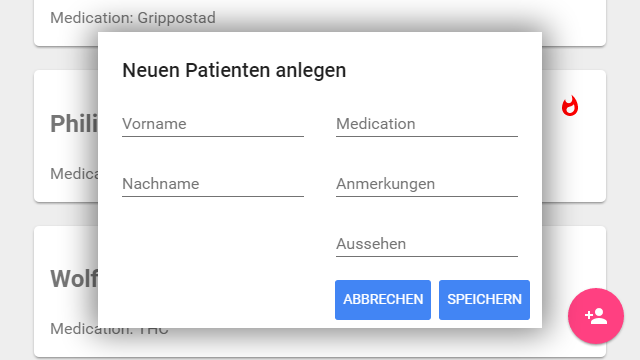
\includegraphics[width=1.0\linewidth]{images/ui/personhinzufuegen}
	\caption{Patient anlegen}
	\label{img:ui/personhinzufuegen}
\end{figure}

\begin{figure}
	\centering
	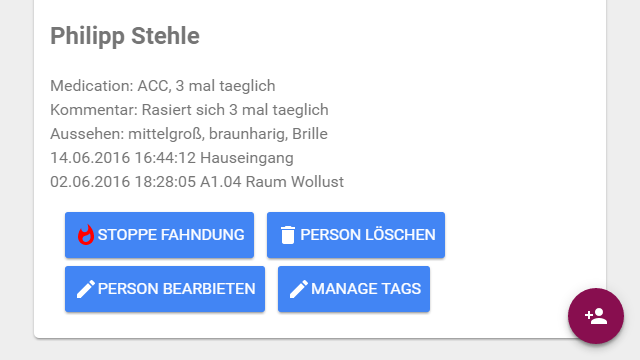
\includegraphics[width=1.0\linewidth]{images/ui/persondetails}
	\caption{Details zu einem Patienten anzeigen}
	\label{img:ui/persondetails}
\end{figure}

\begin{figure}
	\centering
	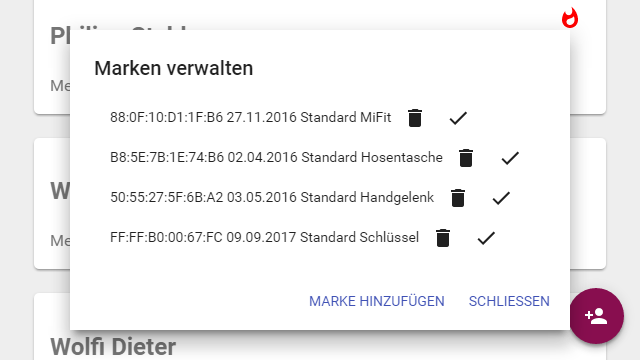
\includegraphics[width=1.0\linewidth]{images/ui/markenverwalten}
	\caption{Marken eine Patienten verwalten}
	\label{img:ui/markenverwalten}
\end{figure}

\begin{figure}
	\centering
	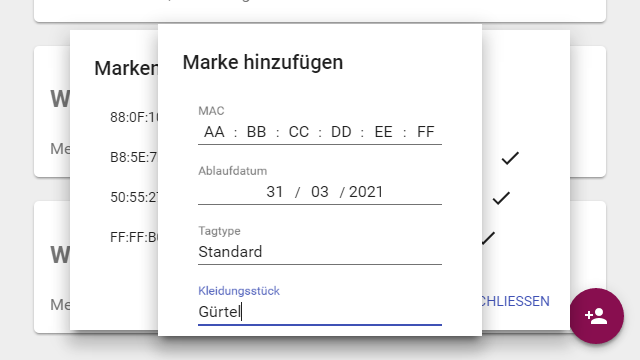
\includegraphics[width=1.0\linewidth]{images/ui/markehinzufuegen}
	\caption{Neue Marken einem Patienten zuordnen}
	\label{img:ui/markehinzufuegen}
\end{figure}

\subsubsection{Administrative Benutzeroberfläche}
In der aktuellen Umsetzung gibt es noch keine Administrative Benutzeroberfläche. Zum Hinzufügen und Löschen von Nutzern steht ein Script zur Verfügung: "/opt/desearch-server/userManagement.py" (vgl. Abbildung \ref{img:userManagement}).\newline
Das Einlernen von neuen Box wird über das in Kapitel \ref{cap:authentifizierung} erwähnte Script durchgeführt.

\begin{figure}
	\centering
	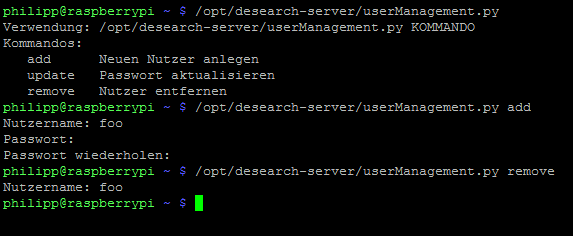
\includegraphics[width=1.0\linewidth]{images/userManagement}
	\caption[Nutzermanagement auf der Zentrale]{Nutzermanagement auf der Zentrale unter der Verwendung des Scripts "/opt/desearch-server/userManagement.py". Das Passwort wird dabei während der Eingabe nicht angezeigt.}
	\label{img:userManagement}
\end{figure}


\subsubsection{Infrastruktur und Netzwerk-Einschränkungen in der Testumgebung}\label{sssec:tunnel}
Die Raspberry Pi's werden in der DHBW Ravensburg am Campus Friedrichshafen zum Testbetrieb installiert. Dabei fungiert ein Pi als Zentrale und die anderen als DeSearch-Boxen, die die Funde an die Zentrale melden. In Tabelle \ref{tab:pis} ist eine Übersicht über alle installierten Raspberry Pi's aufgelistet.
Dazu wurde vom Netzwerkadministrator der DHBW die Erlaubnis eingeräumt, die vorhandene Infrastruktur zu verwenden. Daran geknüpft sind allerdings folgende Bedingungen bzw. Einschränkungen:
\begin{itemize}
	\item Zugriffe aus dem Internet sind nicht erlaubt.
	\item Alle Pi's außer der Zentrale (Slaves) verbinden sich über WLAN unter Verwendung der persönlichen Zugangsdaten mit dem Netzwerk.
	\item Die Zentrale bekommt einen LAN Anschluss und eine feste IP Adresse plus DNS Eintrag zugewiesen.
	\item Ein Verbindungsaufbau zu den Slaves ist nicht möglich - jegliche Kommunikation muss von ihnen initiiert werden.
\end{itemize}
Die letzte Bedingung stellt eine Herausforderung dar, da damit auch kein SSH-Zugriff auf die DeSearch-Boxen möglich ist, der benötigt wird um die DeSearch Anwendung zu aktualisieren, starten oder überwachen.
Dieses Problem kann gelöst werden, da mit der Zentrale ein Gerät im Netzwerk ist, das für alle anderen Pi's und auch die zur Entwicklung und Wartung verwendeten Laptops erreichbar ist. Somit kann über die Zentrale ein Tunnel aufgebaut werden.
Zum Aufbauen des Tunnels bietet sich die Verwendung der SSH Portforwarding Funktion an, da alle beteiligten Geräte bereits für die Verwendung von SSH eingerichtet sind. Eine schematische Darstellung der Vorgehensweise ist in Abbildung \ref{fig:tunnel} zu sehen.
Zum Verbindungsaufbau wurde ein technischer Benutzer mit dem Namen "tunnel" auf der Zentrale angelegt, der sich über SSH und Zertifikat Authentifizierung einloggen kann.
Jeder Slave erhält einen RSA Schlüssel, den er zum Login verwenden kann, und über einen Eintrag in der Crontabelle wird sichergestellt, dass der Tunnel immer offen gehalten wird.
Der Ausgangsport des Tunnels ist dabei für jede DeSearch-Box eindeutig. Soll nun eine Verbindung zu einer Box hergestellt werden, so muss erst eine SSH Verbindung zur Zentrale aufgebaut werden und dort eine SSH Verbindung zum Eingang des Tunnels (localhost plus Tunnel Ausgangport) hergestellt werden.
\begin{table}[h]
	\begin{tabular}{ | p{2,5cm} | p{2,5cm} | p{4cm} | p{6cm} |}
		\hline
		\textbf{Pi-Nummer} & \textbf{Funktion} & \textbf{Installationsort} &  \textbf{Erreichbarkeit} \\ \hline
		3 & Zentrale & Büro Herr Judt & statische IP 141.68.30.39 oder \mbox{Judt-Master.it.ba-ravensburg.de} \\ \hline
		5 & DeSearch-Box & Haupteingang oberhalb der Treppe & Tunnel über Zentrale, Port 19005 \\ \hline
		6 & DeSearch-Box & DHBW-Mensa (Kühlschrank) & Tunnel über Zentrale, Port 19006 \\ \hline
		7 & DeSearch-Box & Container (Raum 603) & Tunnel über Zentrale, Port 19007 \\ \hline
		9 & DeSearch-Box & Eingangsbereich linker Flügel der DHBW & Tunnel über Zentrale, Port 19009 \\ \hline
		10 & DeSearch-Box & Eingangsbereich rechter Flügel der DHBW & Tunnel über Zentrale, Port 19010 \\ \hline
	\end{tabular}
	\caption{Übersicht der Raspberry Pi's mit Funktion, Installationsort und Erreichbarkeit}
	\label{tab:pis}
\end{table}

\begin{figure}
	\centering
	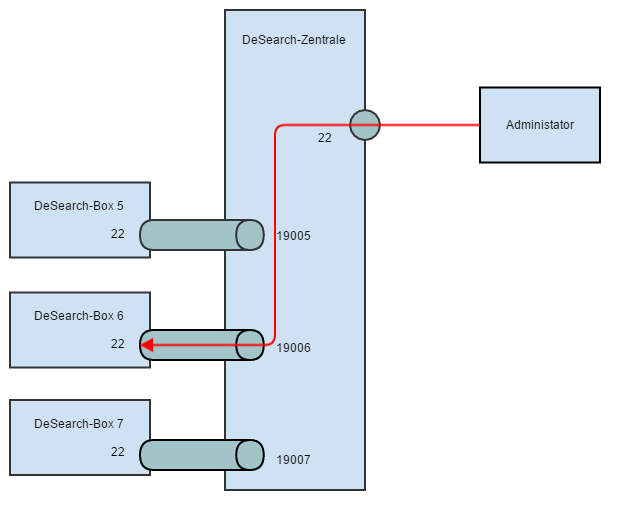
\includegraphics[width=\textwidth]{images/tunnel.png}
	\caption[Schematische Darstellung der Verwendung des SSH Tunnels]{\textbf{Schematische Darstellung der Verwendung des SSH Tunnels} - Beispielhaft ist hier eine Verbindung vom Administrator zur DeSearch-Box 6 dargestellt (roter Pfeil), Quelle: eigene Darstellung}
	\label{fig:tunnel}
\end{figure}


\subsubsection{Installation einer neuen DeSearch-Box in der Testumgebung}\label{sssec:schritte}
Im Folgenden sollen alle Schritte erläutert werden, die für das Einbringen eines neuen Raspberry Pi als DeSearch-Box in das Testsystem durchgeführt werden müssen.
Voraussetzung dabei ist, dass der Pi bereits das Betriebssystem Raspbian vorinstalliert hat und mit einem WLAN- und Bluetooth-Dongle ausgestattet ist.\\
\textbf{Schritt 1: Internetverbindung}\\
Sofern noch nicht geschehen, muss der Raspberry mit dem Internet verbunden werden. Dies kann entweder schon im Testsystem geschehen, oder in der Entwicklungsumgebung in einem anderen Netzwerk. Der Zugriff auf den Raspberry erfolgt bei bereits bestehender Verbindung über SSH, andernfalls wird der Pi über HDMI an einen Monitor angeschlossen und zunächst direkt mit Maus und Tastatur konfiguriert. \\
\textbf{Schritt 2: Software aktualisieren}\\
Zunächst sollten einige unnötige Software-Installationen von Raspbian entfernt werden, da diese sonst bei jedem Update große Datenmengen herunterladen und installieren. Beispielsweise ist LibreOffice und WolframEngine vorinstalliert, wird aber auf der DeSearch-Box nicht benötigt. Mit \texttt{apt-get purge libreoffice* wolfram-engine} und \texttt{apt-get autoremove} werden diese deinstalliert und gelöscht. Anschließend wird die Software mittels \texttt{apt-get update} und \texttt{apt-get upgrade} auf den neuesten Stand gebracht. Hierfür muss der Pi eine Internet-Verbindung haben.\\
\textbf{Schritt 3: Hostname anpassen}\\
Um die DeSearch-Boxen später im Netz voneinander unterscheiden zu können, muss der Hostname des Gerätes angepasst werden. Hierfür wird der Hostname in der Datei \texttt{/etc/hostname} und in der Datei \texttt{/etc/hosts} von \texttt{raspberrypi} auf z.B. \texttt{pi9} geändert. Damit diese Änderung wirkt, muss der Pi neu gestartet werden.\\
\textbf{Schritt 4: Statische IP-Adresse konfigurieren}\\
Falls der Pi im WLAN noch nicht gefunden werden kann, ist die Alternative eine SSH-Verbindung über LAN. Damit diese funktioniert, wird eine statische IP-Adresse auf dem Interface eth0 konfiguriert. Dazu muss ein Eintrag in die Datei \texttt{/etc/network/interfaces} gemacht werden:\\
\texttt{auto eth0\\
	allow-hotplug eth0\\
	iface eth0 inet static\\
	address 192.42.42.2 // Dies ist die beispielhafte statische IP-Adresse\\
	netmask 255.255.255.0}\\
\textbf{Schritt 5: Netzwerkzugriff in der Testumgebung}\\
Je nach Vorgehensweise kann dieser Schritt auch bereits als erster Schritt erfolgen. Um die Zugangsdaten für das WLAN-Netzwerk der DHBW zu konfigurieren, muss die Datei \texttt{/etc/wpa\_supplicant/wpa\_supplicant.conf} bearbeitet werden. Hier wird der Eintrag (beispielhaft für das DHBW-Netzwerk) folgendermaßen angelegt:\\
\texttt{network=\{\\
	\tab ssid="DHBW-STUDENT"\\
	\tab key\_mgmt=WPA-EAP\\
	\tab identity="<Nutzername>"\\
	\tab password="<Passwort>"\\
	\}}\\
\textbf{Schritt 6: Tunnel zur Box einrichten}\\
Für den Zugriff auf die neue DeSearch-Box muss ein SSH-Tunnel von der Zentrale aus hergestellt werden(siehe auch Kapitel \ref{sssec:tunnel}). Hierfür wird im home-Verzeichnis zunächst die Datei \texttt{tunnel.sh} angelegt und mit folgendem Inhalt gefüllt:\\
\texttt{\#!/bin/bash\\
	/usr/bin/autossh -i /home/pi/tunnel -fN -R 19005:localhost:22 141.68.30.39}\\
Zudem wird die Datei \texttt{tunnel} im home-Verzeichnis erstellt, in der der Private Key des tunnel-Users auf der Zentrale abgelegt wird. Das Tunnel-Skript greift dann beim Aufbau des ssh-Tunnels auf diese Datei als Key zu. Nachdem diese beiden Dateien erstellt wurden, müssen die Berechtigungen angepasst werden. Mit \texttt{chmod 755 tunnel.sh} und \texttt{chmod 600 tunnel} wird das Skript ausführbar und nur der Pi-User hat Lesezugriff auf den Private Key. Als nächstes wird das tunnel-Skript in einen Cronjob eingefügt, damit der Tunnel immer selbständig aufgebaut wird, auch nach einem reboot des Systems. Hierfür ruft man \texttt{crontab -e} auf und fügt folgende Zeile ein: \texttt{@reboot /home/pi/tunnel.sh}\\
Als letzten Schritt sollte überprüft werden, ob das Tool autossh installiert ist. Andernfalls wird es mit \texttt{apt-get install autossh} installiert.\\
\textbf{Schritt 7: DeSearch-Software installieren}\\
Nachdem die Verbindung zu der Box und die Infrastruktur gesichert sind, kann nun die DeSearch-Software auf der Box installiert werden. Zunächst wird die Datei\\ \texttt{/etc/apt/sources.list.d/desearch.list} angelegt. In diese Datei fügt man folgende Zeile ein: \texttt{deb https://www.philipp1994.de/apt/ vivid desearch}. Somit wird festgelegt, aus welcher Quelle die desearch-Software bezogen wird. Der angegebene Server ist beispielhaft für das Testsystem und muss für die Produktivnutzung geändert werden. Anschließend wird mit \texttt{apt-get install apt-transport-https} die Installation über HTTPS ermöglicht. Dafür wird der Public Key des Quellservers benötigt, der mit\\ \texttt{wget https://philipp1994.de/philipp1994.de.gpg} heruntergeladen werden kann. \texttt{apt-key add philipp1994.de.gpg} installiert diesen Key, sodass die .gpg-Datei anschließend gelöscht werden kann. Ein Aufrufen von \texttt{apt-get update} lädt nun die verfügbaren Software-Updates für die DeSearch-Software herunter. Installiert wird die Software durch \texttt{apt-get install desearch-client}. Im Installationsprozess muss die Box-Nummer und die Service-URL angegeben werden (siehe Abbildungen \ref{fig:installation1} und \ref{fig:installation2}).
\begin{figure}
	\centering
	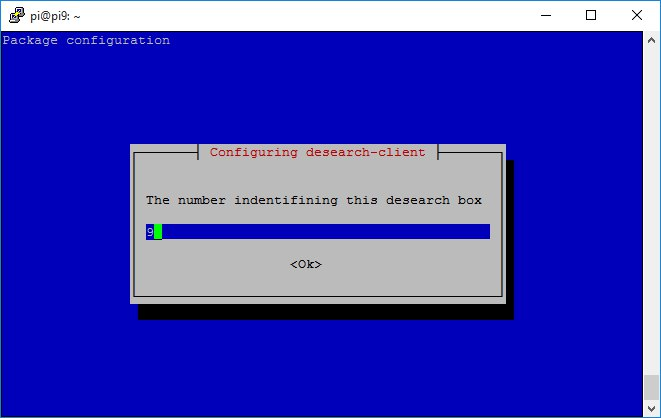
\includegraphics[width=\textwidth]{images/installation1}
	\caption[Eingabe der Box-Nummer bei Installation der DeSearch-Software]{Installationsprozess der DeSearch-Software, hier wird die Box-Nummer eingegeben. Quelle: eigene Darstellung}
	\label{fig:installation1}
\end{figure}
\begin{figure}
	\centering
	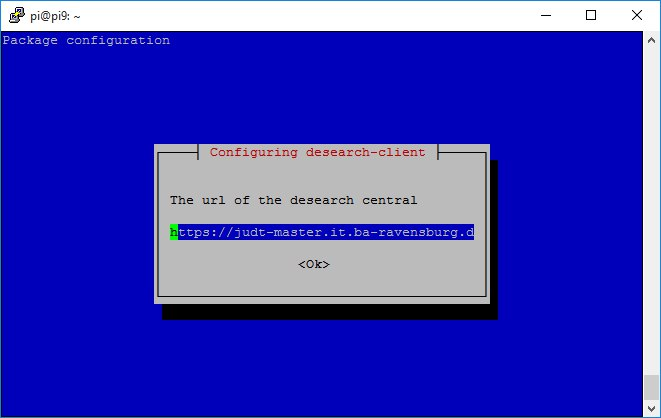
\includegraphics[width=\textwidth]{images/installation2}
	\caption[Eingabe der Service-URL bei Installation der DeSearch-Software]{Installationsprozess der DeSearch-Software, hier wird die Service-URL eingegeben. Quelle: eigene Darstellung}
	\label{fig:installation2}
\end{figure}  
Eine erfolgreiche Installation kann mit \texttt{service desearch-client status} überprüft werden. Hier sollte der Status \enquote{active(running)} angezeigt werden (siehe auch Abb. \ref{fig:systemctl-status}).\\
\textbf{Schritt 8: Bekanntmachen der Box an der Zentrale}\\
Im letzten Schritt müssen die neue DeSearch-Box und die Zentrale ihre Keys austauschen, um eine sichere Kommunikation zu ermöglichen (vgl. Kapitel \ref{cap:authentifizierung}). Hierfür muss das python-Skript \texttt{/opt/desearch-client/keyExchange.py} ausgeführt werden. Gleichzeitig muss auf der Zentrale das python-Skript \texttt{/opt/desearch-server/keyExchange.py} ausgeführt werden. So werden die Keys auf Server und Client generiert (dies kann auf einem Raspberry Pi einige Zeit dauern) und anschließend muss der User die Hash-Werte der Keys auf Zentrale und Box vergleichen. In Abbildung \ref{fig:keyEx} ist der Key-Exchange auf einer DeSearch-Box zu sehen. 
\begin{figure}
	\centering
	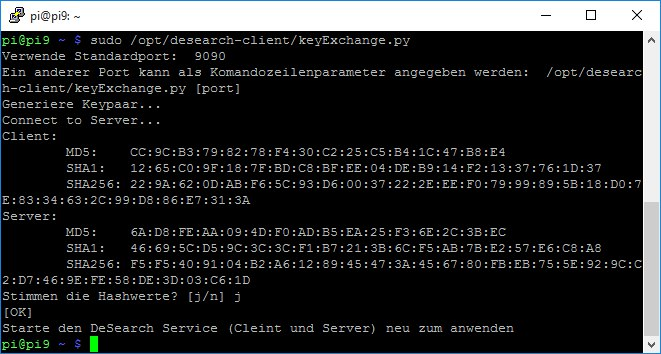
\includegraphics[width=\textwidth]{images/keyExchange}
	\caption[Key-Exchange zwischen DeSearch-Box und Zentrale]{Key-Exchange zwischen DeSearch-Box und Zentrale, hier wird der User aufgefordert, die Hash-Werte zu vergleichen. Quelle: eigene Darstellung}
	\label{fig:keyEx}
\end{figure}
Nach der Bestätigung ist die Box nun im System bekannt und kann sicher mit der Zentrale kommunizieren.

\nomenclature{LAN}{\textbf{L}ocal \textbf{A}rea \textbf{N}etwork}
\nomenclature{WLAN}{\textbf{W}ireless \textbf{LAN}}
\nomenclature{HTTP}{\textbf{H}yper\textbf{T}ext \textbf{T}ransfer \textbf{P}rotocol}
\nomenclature{HTTPS}{\textbf{H}yper\textbf{T}ext \textbf{T}ransfer \textbf{P}rotocol \textbf{S}ecure}
\nomenclature{ARM}{\textbf{A}dvanced \textbf{R}ISC \textbf{M}achines}
\nomenclature{RISC}{\textbf{R}educed \textbf{I}nstruction \textbf{S}et \textbf{C}omputer}
\nomenclature{CPU}{\textbf{C}entral \textbf{P}rocessing \textbf{U}nit}
\nomenclature{SD-Karte}{\textbf{S}ecure \textbf{D}igital Memory \textbf{Card}}
\nomenclature{URL}{\textbf{U}niform \textbf{R}esource \textbf{L}ocator}
\nomenclature{FTP}{\textbf{F}ile \textbf{T}ransfer \textbf{P}rotocol}
\nomenclature{SQL}{\textbf{S}tructured \textbf{Q}uery \textbf{L}anguage}
\nomenclature{ORM}{\textbf{o}bject \textbf{r}elational \textbf{m}apping}
\nomenclature{SSH}{\textbf{S}ecure \textbf{Sh}ell}
\nomenclature{GUI}{\textbf{G}raphical \textbf{U}ser \textbf{I}nterface}
\nomenclature{CA}{\textbf{C}ertificate \textbf{A}uthority}
\nomenclature{MITM Attake}{\textbf{M}an-\textbf{i}n-\textbf{t}he-\textbf{m}iddle Attake}